\ifdefined\included
\else
\setcounter{chapter}{1} %% Numéro du chapitre précédent ;)
\dominitoc
\faketableofcontents
\fi

\chapter{A Human Aware Task Planner Emulating Human Decisions and Actions (HATP/EHDA)}
\chaptermark{HATP/EHDA}
\label{chap:2}
\minitoc

\section{Introduction}

I was introduced to the field of task planning the work of a PhD student from my lab, Guilhem Buisan. I slightly contributed to the original version and then proposed two extensions of his work. Yet, Guilhem mainly designed and implemented this novel human-aware task planning approach dedicated to HRI which plans the robot's actions while estimating and emulating the human decisions and actions, namely HATP/EHDA. 

We believe this planning approach suits well the needs of HRI scenarios, and thus, it became a laboratory to address relevant challenges of task-planning for HRC. 
Two of my main contributions consist of addressing such challenges and then implementing the solutions as extensions of HATP/EHDA.   
As a consequence, it is important to understand this work well, both its motivation and methods, before introducing my proper contributions. This section introduces, motivates and explains the HATP/EHDA approach as a background to the other chapters. 
Naturally, a detailed description of this prototypical planner is already given in Buisan's thesis~\cite{thesisBuisan21}. Thus, large parts of this section are directly retrieved from Buisan's thesis, but they are important to have in mind. Some notations are adapted to match my contributions' descriptions in the next chapters. 

\subsection{Rationales}

HATP/EHDA has been developed to try to satisfy several objectives: 
\begin{enumerate}
    \item \textbf{Plan without assuming a prior shared goal.} In HRI scenarios, the robot and the human do not always share a goal. The robot can for example plan to perform a task around humans that are not involved at first, or it may be requested by a human to do a task without wanting to take a part in it. HATP/EHDA can balance between integrating the sharing of a goal with a human (assumed to be collaborative) in the plan and making the robot do the task alone, or integrate the eventuality to ask for punctual human help. 

    \item \textbf{Model the human decision processes.} When taking part in a task, a human (assumed willing to collaborate with the robot) will also plan to reach their (potentially shared) goal. HATP/EHDA must be able to account for this to provide plans that are expected and explainable by the human partner.

    \item \textbf{Help the human decisions, but not compel them.} Unlike HATP, HATP/EHDA should account for human flexibility in their decision. While by modeling the human decision processes it is possible to narrow down the possible human actions, the generated plans must be able to help the supervision (execution of the plan) to avoid replanning or repairing during the execution by considering several human actions.

    \item \textbf{Model the potential human reactions.} It is possible to predict that the human may react to some situations, interrupting or helping their current task. Two causes have been identified for these reactions. First, they can ensue from some specific world states, that have been perceived and interpreted by the human. Then, they can also originate from explicit communications issued by the robot. These communications can either be a belief alignment, updating the human knowledge and impacting their decisions; a request to perform a specific action or a request to help the robot along with a shared goal, needing the human to plan for it.

    \item \textbf{Act and decide on the different agents' beliefs.} It is important to be able to represent actions as having different effects on the beliefs of the robot or the human. Indeed, some robot actions are partially or not observable by the human, when performing them, the human has no way of knowing the complete new world state. Besides, these effects and their observability often depend on the current world state, which representation must be supported in the planner. Then, decisions made while planning may require reasoning on both the robot and the human beliefs. This is especially the case with communication actions aiming at aligning knowledge or asking questions for example. Finally, some actions of pure decision have no direct effect on the world, but only on the internal beliefs of the agents. For example, observation actions will only update the beliefs of the agent doing it.

    \item \textbf{Decide not only on the world state but also on the decision processes of the agents.} Some decisions made during the planning process require access not only to the beliefs of the agents representing the world state, but also to the estimation of their planning processes. For example, the decomposition of a task by the robot may be impossible if some other task is already performed in its partial plan. Other decisions may also need the estimation of the human current planning process. For example, if it has been estimated earlier in the plan that the human will perform a certain decomposition of a task, the planner would assign a complementary task to the robot.

    \item \textbf{Adapt to the human experience, trust and preferences.} We also want the planning process to be adjusted depending on the actual human it is planning with. It must perform its plan search differently whether the human has the habit of performing this particular task with the robot or not. Moreover, the human model can be adjusted to the trust the human has in the robot and to their preferences.

\end{enumerate}

\subsection{Running example}

\begin{figure}
    \centering
    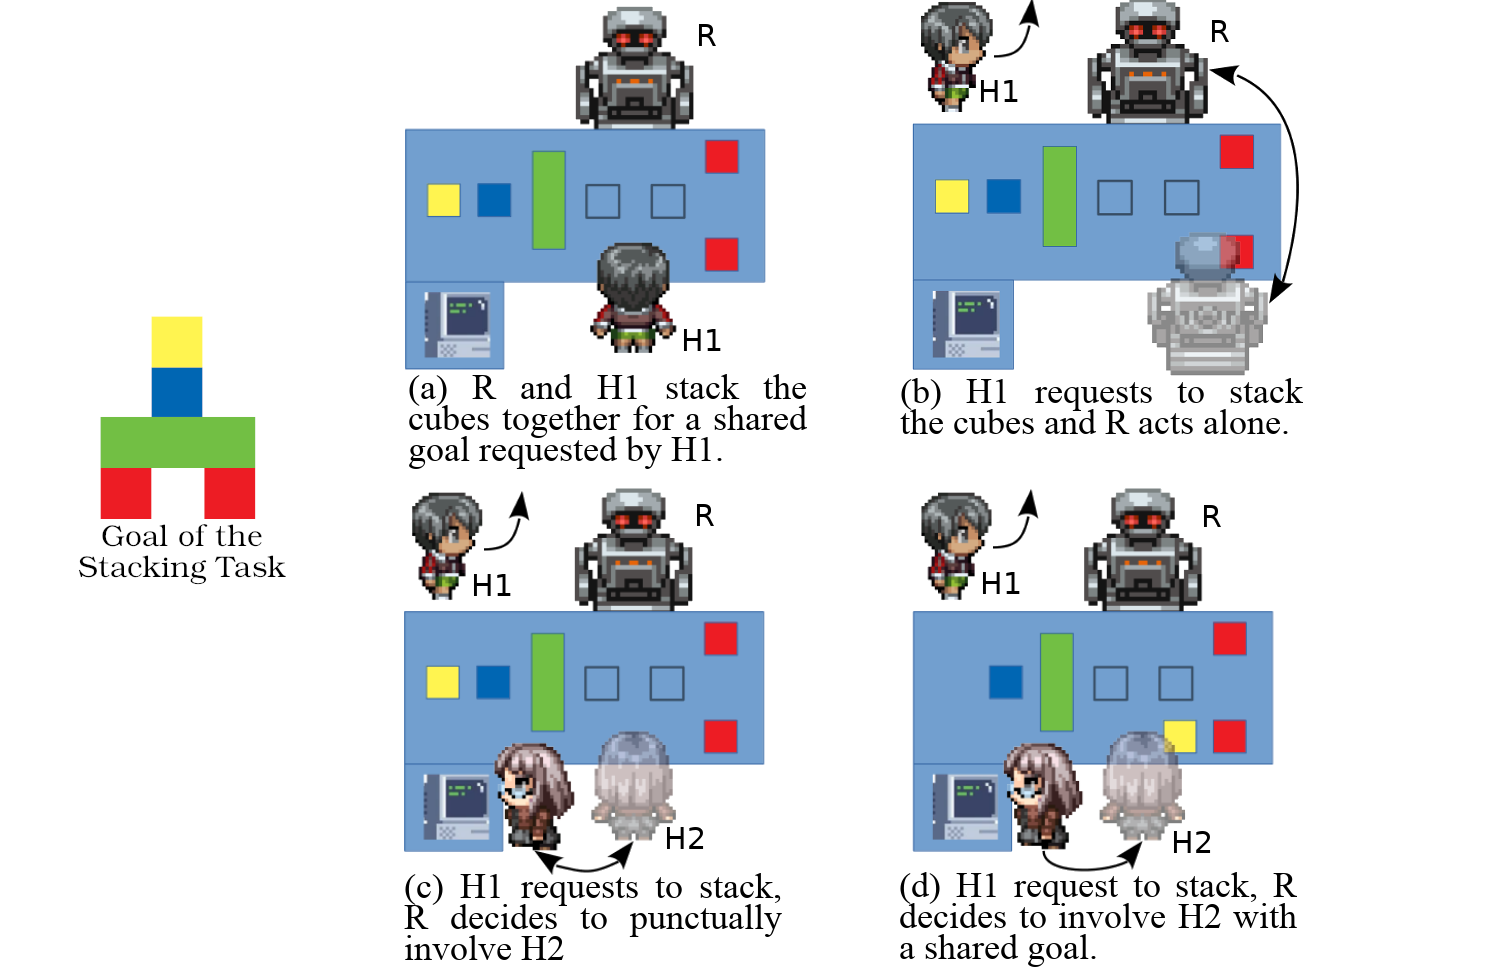
\includegraphics[width=\linewidth]{images/Chapter2/scenarios.png}
    \caption{Cube stacking scene: A different plan is selected for each scenario, involving nearby humans in the less disturbing way possible}.
    \label{fig:scenarios}
\end{figure}

To highlight the potential of our approach we present as an example a cube stacking scene. The scene is depicted in four different scenarios in \ref{fig:scenarios}. The goal consists of stacking the colored cubes on the empty marks to match the colors on the left of the figure. All cubes placed in the middle of the table are reachable from anywhere. However, when close to one side a cube is only reachable from this specific side.

\section{Related work}

\subsection{HATP}
The Hierarchical Agent-based Task Planner (HATP) proposes a hierarchical approach to multi-agent task planning. This HTN-based planner is able to elaborate a multi-agent plan based on a single HTN tree. Moreover, it maintains one beliefs base per agent allowing to write task decomposition rules and actions preconditions and effects in any agent beliefs base. Finally, HATP also computes costs for the plans found based on action costs and predefined social rules. However, HATP assumes that a shared goal has been established between the human and the robot prior to the planning process and that the generated plan will be shared with the human before the execution. Indeed, HATP does not represent the human as an agent having a separate decision process that may lead to diverging plans without robot communication. Hence, any deviation of the human from their generated stream of action either needs supervision to perform repair action or to request for a replanning. Such an approach can work well but assumes that communication can easily be done at any point of the plan.  

\subsection{Other human-aware task planner}

\textbf{TODO: List planners and approaches, general and some specific ones? maybe not, already done in next chapters}

\section{Problem Specification and Solution}

\subsection{Problem Specification}

The notations from Buisan's thesis have been adapted to match the notations in this thesis and ease readers' comprehension. We start from classical planning formalization.

We consider a \textit{classical planning domain} (\textit{state-transition system}) $\Sigma = (S, A,\gamma)$, s.t., $S$ is a finite set of states in which the system may be, $A$ is a finite set of actions that the actors may perform, $\gamma: S \times A \rightarrow S$ is a state-transition function. Each state $s \in S$ is a description of the properties of various objects in the planner's environment~\cite{naubooks0014222}. 

To represent the objects and their properties, we will use two sets $B$ and $X$: $B$ is a set of names for all the objects, plus any mathematical constants representing the properties of those objects. $X$ is a set of syntactic terms called state variables, s.t. the value of each $x \in X$ depends solely on the state $s$.

A \textit{state-variable} over $B$ is a syntactic term $x = sv(b_1, ..., b_k)$, where $sv$ is a symbol called the state variable's name, and each $b_i$ is a member of $B$ and a parameter of $x$. Each state variable $x$ has a range, $\textit{Range}(x) \subseteq B$, which is the set of all possible values for $x$.


Here is the description of the sets $B$ and $X$ for the stacking example given in the introduction:
{\small
\begin{align*}
&B           = Entities \cup Locations \cup TableZones \cup Booleans \cup \{\textsf{nil}\} \\
&\quad Entities    = Agents \cup Cubes\\
&\quad Agents      = \{ \textsf{R}, \textsf{H} \} ~~ \backslash\backslash~\textsf{R}:robot,~\textsf{H}:human\\
&\quad Cubes     = \{ \textsf{red1}, \textsf{red2}, \textsf{green1}, \textsf{blue1}, \textsf{yellow1} \}\\
&\quad Locations     = \{ \textsf{base1}, \textsf{base2}, \textsf{bridge}, \textsf{top1}, \textsf{top2} \}\\
&\quad TableZones     = \{ \textsf{middle}, \textsf{side\_h}, \textsf{side\_r} \}\\
&\quad Booleans    = \{ \textsf{true},\textsf{false} \}\\
&\\
&X = \{ at(e), holding(a), solution(l) ~ | ~ e \in Entities, a \in Agents, l \in StackLocations\}\\
&\quad \textit{Range}(holding(a) ~|~ a \in Agents) = Cubes \cup \{\textsf{nil}\} \\
&\quad \textit{Range}(at(a) ~|~ a \in Agents) = \{ \textsf{side\_h}, \textsf{side\_r} \}\\
&\quad \textit{Range}(at(c) ~|~ c \in Cubes) = TableZones \cup Locations\\
&\quad \textit{Range}(solution(l) ~|~ l \in StackLocations) = Cubes \\
\end{align*}
}

% \vspace{-1cm}

\textbf{TODO: Make proper definitions? Here to much lost in the text... and easier in next chapter to say ``we redefine def.x''}

A \textit{variable value assignment} function over $X$ is a function $val$ that maps each $x_i \in X$ into a value $z_i \in$ $\textit{Range}(x_i)$. With $X = \{ x_1, ..., x_n \}$, this function can be written as a set of assertions: $val = \{ x_1=z_1, \ldots, x_n=z_n \}$. 

An \textit{action} is a tuple $\alpha = (\textit{head}(\alpha), \textit{pre}(\alpha), \textit{eff}(\alpha))$ where $\textit{head}(\alpha)$ is a syntactic expression of the form $\textit{act}(z_1, ..., z_k)$ where $act$ is a symbol called the \textit{action name} and $z_1,...,z_k$ are variables called parameters. $\textit{pre}(\alpha) = \{ p_1, ..., p_m \}$ is a set of preconditions, each of which is a literal. And $\textit{eff}(\alpha) = \{ e_1, ..., e_n \}$ is a set of effects, each of which is an expression of the form: $sv(t_1, ..., t_j) \leftarrow t_0$ with $t_0$ being the value to assign to the state variable $sv(t_1, ..., t_j)$. We note $\textit{agt}(\alpha)$ the agent performing the action $\alpha$.

The problem specification of HATP/EHDA is a pair of two distinct human and robot models as follows: $P = \{ \mathcal{M}^H, \mathcal{M}^R \}$. Each model $\mathcal{M}^\varphi$, for an agent $\varphi$, comprises the following:
\begin{itemize}
    \item \textbf{Name} ($name^{\varphi}$): being the name of the agent. Hence, either ``robot'' or ``human''.
    
    \item \textbf{Beliefs} ($val^{\varphi}$): estimation of the world state from the agent's perspective.
    
    \item \textbf{Agenda} ($d^{\varphi}$): capturing the personal and/or shared goals of the agent, currently implemented as a task list/sequence but could be generalized to partially ordered task networks.
    
    \item \textbf{Partial Plan} ($\pi^{\varphi}$): storing the current partial plan on an agent. This is empty at the beginning and filled during the planning process.
    
    \item \textbf{Action Model} ($\Lambda^{\varphi}$): encoding the capabilities of the agent and used to estimate the next actions of the agent given a goal and a world state. Here described by a hierarchical task network (HTN) and thus a set of operators and methods. 
    
    \item \textbf{Triggers} ($Tr^{\varphi}$): describes the reactions the agent may have which might update their agenda. That is, the agent may react to a specific world state, event sequence, or an explicit communication. For instance,  consider a scenario where suddenly another agent is handing over an object to the agent. This event has nothing to do with the agent's goal, and thus, the next agent action extracted from the Action Model might not consider the other agent. However, a natural reaction to this situation is to grab the handed object. Thanks to the Triggers mechanic, we can in an automated way estimate that whatever the agent was doing, when being handed an object the agent will grab it.  
\end{itemize}

Note that most of the models' elements are static during the planning process. Only the Beliefs ($val^{\varphi}$), the Agenda ($d^{\varphi}$) and the Partial Plan ($\pi^{\varphi}$) of each agent evolve during the planning process. That is why we define specifically an \textbf{agent state} which is part of the agent model:
$\sigma^{\varphi} = \{ val^{\varphi}, d^{\varphi}, \pi^{\varphi} \}$. 
And thus, the agent model can be written as $\mathcal{M}^{\varphi} = \{ name^{\varphi}, \sigma^{\varphi}, \Lambda^{\varphi}, Tr^{\varphi} \}$.


The planner uses two agent models, one for the human and one for the robot. Despite their identical structure, there is a fundamental difference between the two models: one is a controllable agent and not the other. Indeed, the human model is only used to speculate the human decisions and actions in given situations. 
Then, the robot model is used to plan the robot's actions according to the estimated human actions.
Note that human decisions can still be influenced by the robot's actions, but they cannot be compelled.
It's also important to remember that the two agents are not equivalent, the robot agent's role is to help, assist and facilitate humans, and thus, to synthesize pertinent, legible and acceptable behavior.


A \textit{state}, or \textit{planning state}, $s_i \in S$ is a tuple composed of two agent states $s_i = ( \sigma^{H}_i, \sigma^{R}_i )$.
The state of the world from the perspective of the robot is captured by the variable value assignment function $val^R_i \in \sigma^{R}_i$. Since the planner is assumed to be part of the robot, the beliefs of the robot are assumed to be the ground truth, and thus, are sometimes noted as $val_i$. 
Similarly, $val^H_i \in \sigma^{H}_i$ represents the estimation of $val_i$ from the perspective of the human, also referred to as the estimated human beliefs.
We say that a state $s_i \in S$ contains \textit{false beliefs}, or \textit{belief divergences}, if $\exists x_j \in X, val^H_i(x_j) \neq val^R_i(x_j)$. 
Be careful not to get confused, a \textit{state} is a state in which the planning problem is while being solved, and each \textit{state} is connected to other states through agent actions. Where the \textit{beliefs} are the state of the world from the perspective of an agent, which is part of the \textit{planning state}.
The other elements in the two agent states, namely the agendas and partial plans, indicate respectively what each agent still has to do and which actions they already performed. 

For our example, the initial state $s_0$ would be as follows: 


{\small
\begin{align*}
&s_0 = \{\sigma^R_0, \sigma^H_0\} \\
&\quad \sigma^R_0 = \{ val^R_0, d^R_0, \pi^R_0 \}, \quad \sigma^H_0 = \{ val^H_0, d^H_0, \pi^H_0 \} \\
&\quad d^R_0 = \{ Stack \}, \quad d^H_0 = \{  \} \\
&\quad \pi^R_0 = \pi^H_0 = \{  \} \\
&\quad val^R_0 = val^H_0 = \{at(\textsf{R}) = \textsf{side\_r},~at(\textsf{H}) = \textsf{side\_h}, ~at(\textsf{red1}) = \textsf{side\_r}, \\
&\quad \quad \quad at(\textsf{red2}) = \textsf{side\_h}, ~at(c) = \textsf{middle} ~|~ c \in Cubes\backslash\{ \textsf{red1}, \textsf{red2} \}, \\
&\quad \quad \quad holding(\textsf{R}) = holding(\textsf{R}) = \textsf{nil}, \\
&\quad \quad \quad solution(\textsf{base1}) = \textsf{red}, ~solution(\textsf{base2} = \textsf{red}), ~solution(\textsf{bridge} = \textsf{green}),   \\
&\quad \quad \quad solution(\textsf{top1}) = \textsf{blue}, ~solution(\textsf{top2} = \textsf{yellow}) \}  \\
\end{align*}
}

Note that $d^H_0$ is empty except in scenario (a) where H1 establish a shared goal. Also, for legibility reasons the sets $B$ and $X$ have been slightly modified because in fact the cubes are explicitly associated to colors which are used in the task decompositions. Hence, the solution is simply expressed using the colors and not the cube names. Finding the exact cube to place is described in the action models.

The process of estimating the next actions that an agent $\varphi \in Agents$ is likely to perform in a state $s_i \in S$ will be detailed later. Meanwhile, when refining the agent's agenda $d^{\varphi}$ based on its belief $val^\varphi_i$, we obtain a \textit{refinement} as follows $\textit{ref}(d^\varphi_i, val^\varphi_i)= \{ (a_1,d_1),...,(a_j,d_j) \}$. 
A \textit{refinement} contains a tuple for each estimated possible action $a_j$ and the associated new agenda $d_j$ after being refined. 

In our cooking example, we obtain the following refinement if the starting agent is the human:\\
{\small
$\textit{ref}(d^H_0, val^H_0) = \{ (add\_salt(),d_1), (move\_to(\textsf{kitchen}),d_2) \}$
}

The execution of an action in HATP/EHDA is known by both agents, and thus, for both beliefs we have $\forall x \in X$: 
\begin{equation}
    val_{i+1}(x) = \left\{ 
    \begin{array}{ll}
        w, & \mbox{if} ~ x \leftarrow w \in \textit{eff}(a)   \\ 
        val_i(x), & \mbox{otherwise}
    \end{array}\right.
\end{equation}


\subsection{Solution}
\textbf{TODO: develop and add figure}

AND/OR Tree resulting in a robot policy. Add figure of AND/OR Tree, we plan in a turn taking fashion where each human action is an AND edge and each robot action is a OR edge, and nodes planning states (beliefs + agendas).



\section{Exploration}

To start planning, HATP/EHDA must be given the two action models (the robot and the human HTNs), the initial beliefs of both agents (which can differ) and the initial agenda of both agents. The initial agenda of the robot represents the task to decompose, while the agenda of the human represents any task the human is estimated to be commited to. If a shared goal has been established prior to planning between the robot and the human (\textit{e.g.} the human asking to perform a task with the robot), the agenda of both agent will be filled with the same task.

The planning process is done in three parts: (1) First, both HTNs are explored in a turn taking fashion, resulting in a valid joint plans tree. (2) Then, based on this tree, robot actions are selected according to action, plan-wide and social costs, resulting in a conditional plan, where at each step multiple human actions can be performed but only one robot action is set. (3) Finally, causal and threat links are added between actions of the conditional plan to ease its execution.

The robot HTN exploration is a pretty standard depth-first algorithm. The first task $\lambda$ from its agenda $d^R$ is popped, then if it is an abstract task $\lambda \in Ab$, all the applicable methods are applied, and their results are prepended to the agenda, thus giving new agents state (with the same beliefs as the previous ones but with the robot agenda updated) and branching our search space. We recursively iterate with the new task popped from the new robot agenda. Eventually, the popped task will be a primitive one $\lambda \in Op$, its function will then be applied to the currently explored agent states. If it returns \textit{false} ($\bot$), the action is not applicable, and the exploration backtracks to another decomposition of an abstract task. However, if the action is applicable (returns a new agents state), the action is added to the robot plan and the triggers are run for each agent, updating their agenda if necessary. Then, the human HTN is queried to get their possible next actions from this new agents state. The possible actions found are added to the human plan, and, for each possible new agents state, we apply the triggers of each agent then we continue the robot HTN exploration. This exploration continues until the robot agenda is empty, or all the branches return \textit{false}. The HTNs exploration process is summarized on Fig.~\ref{fig:HATPEHDA_planning_process}.

\begin{figure}
    \centering
    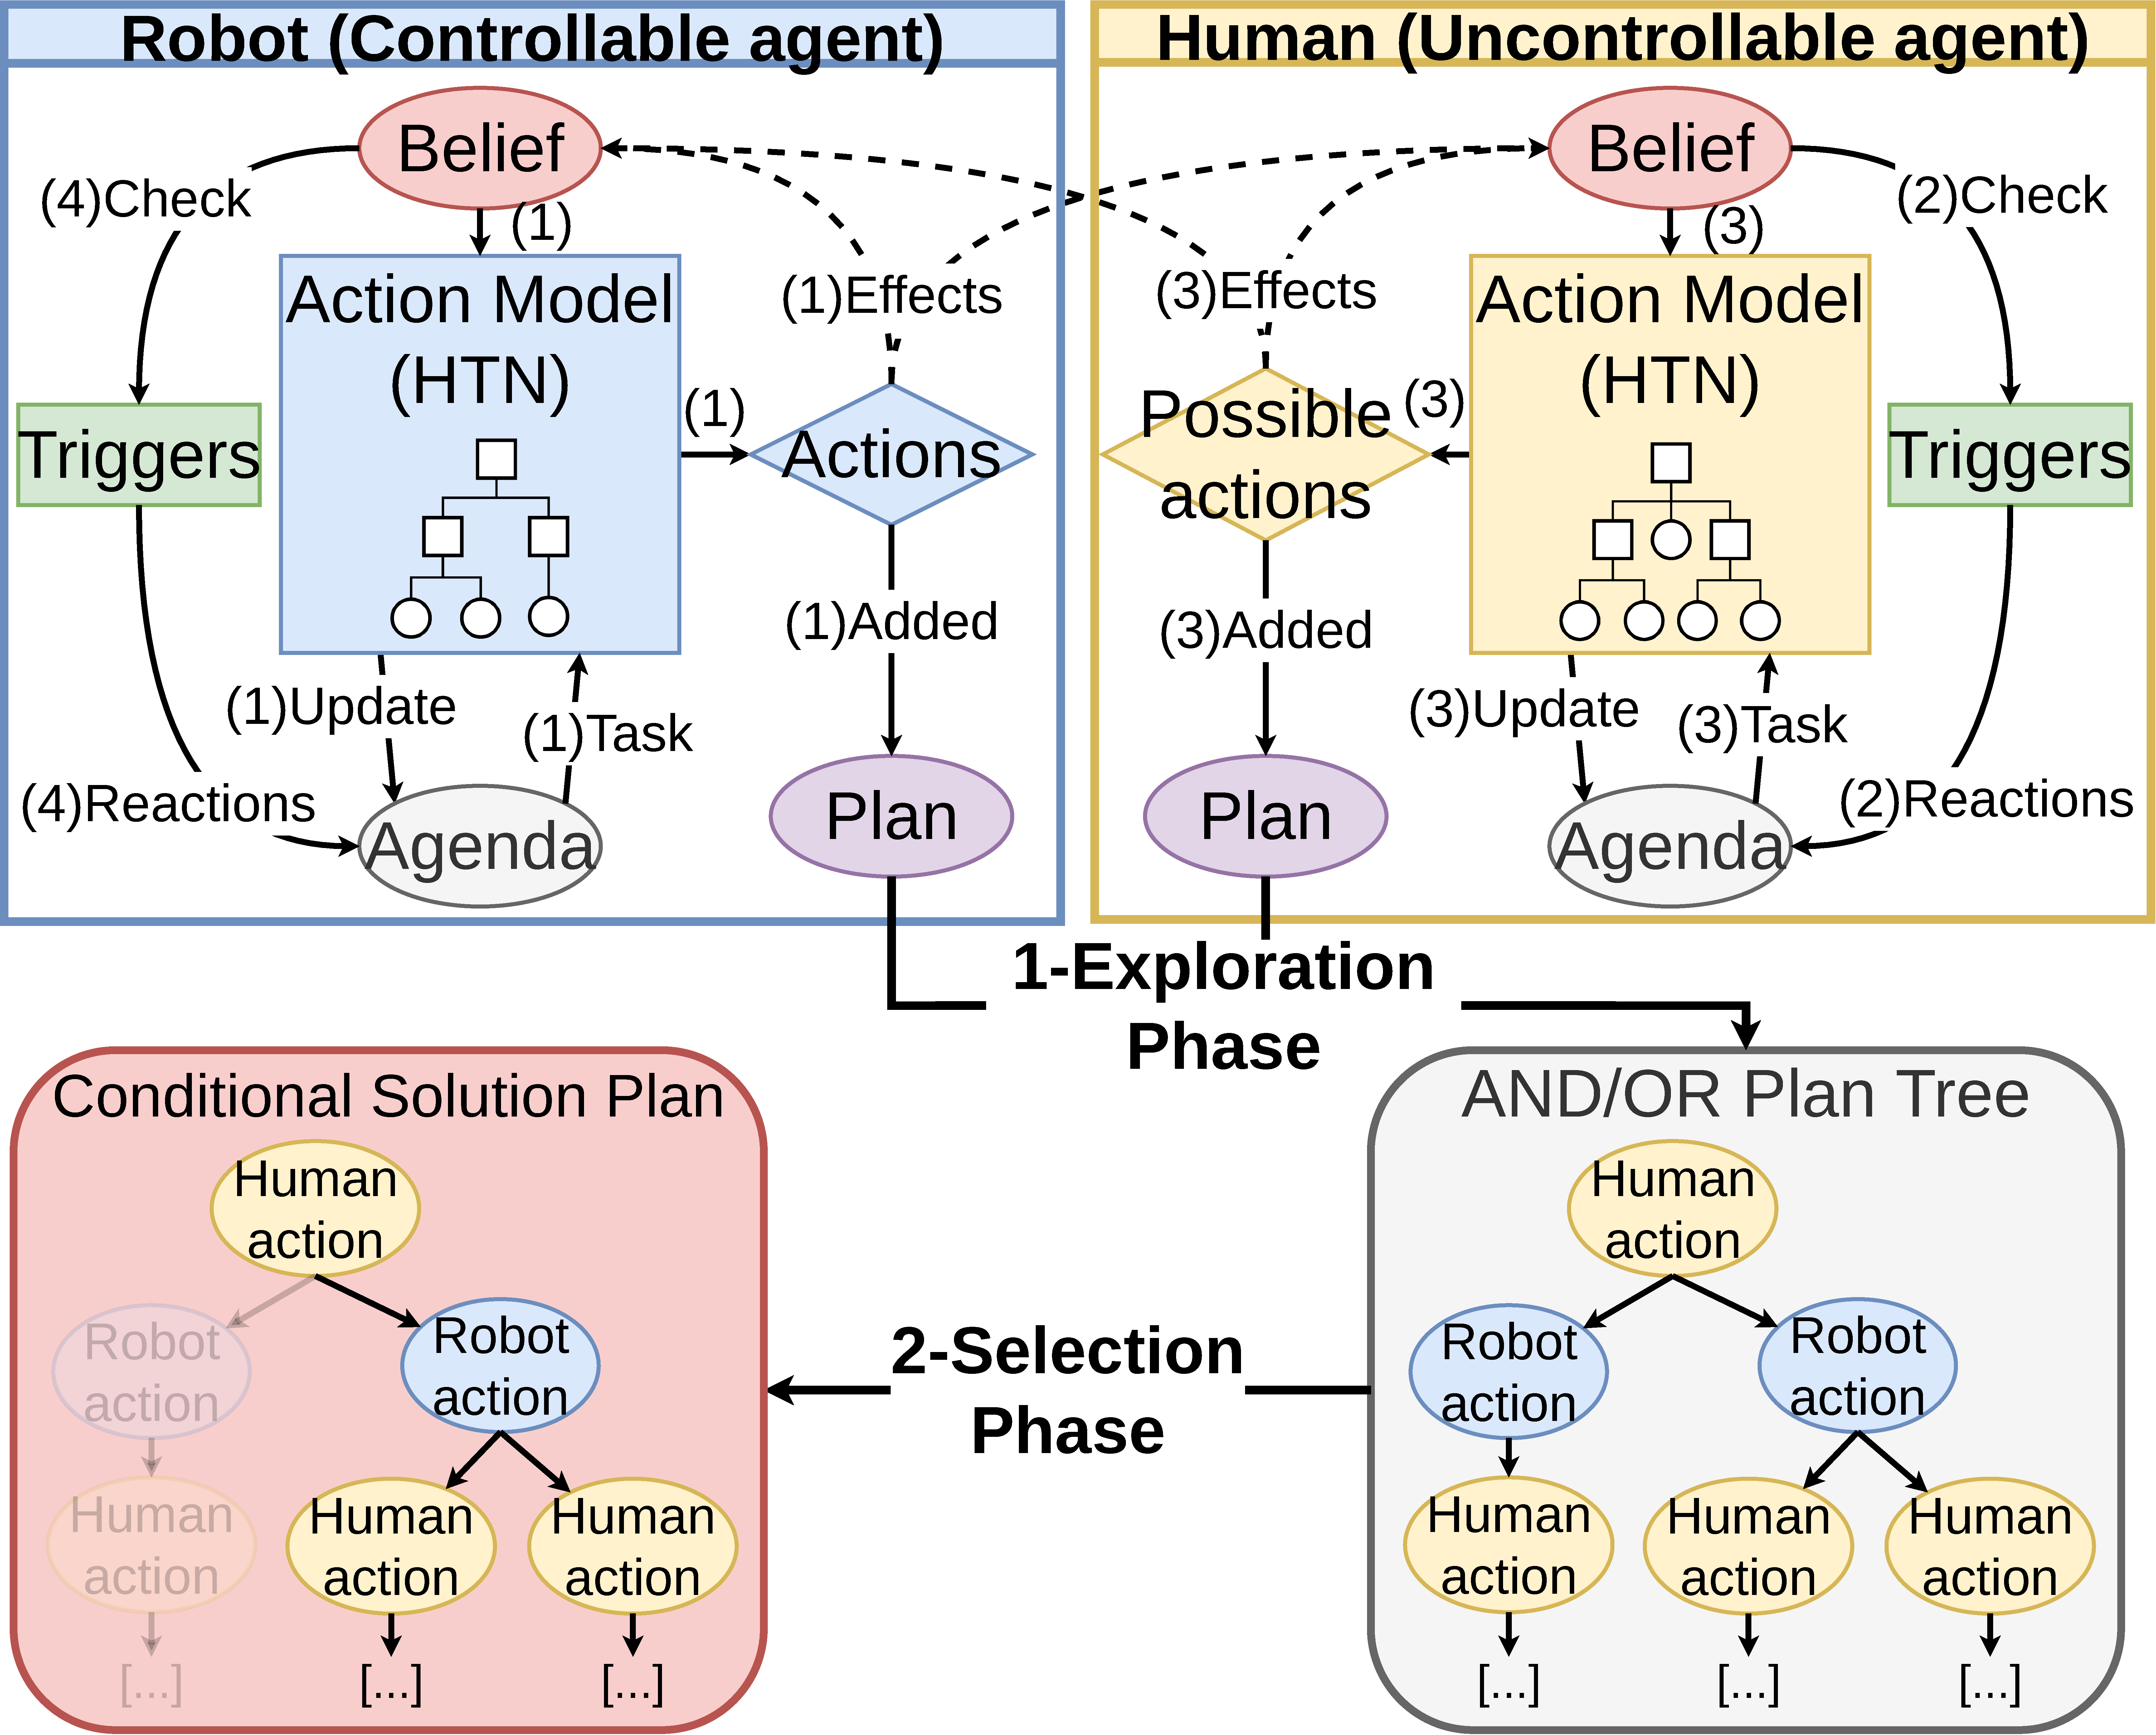
\includegraphics[width=0.8\linewidth]{images/Chapter2/HATPEHDA_planning_process.pdf}
    \caption{The HTNs exploration consists in iterative loops of four steps : (1) Get possible robot actions from the robot HTN, add them in the plan and apply their specific effects on the H \& R beliefs, (2) Check Triggers and add the reactions in the corresponding agendas, (3) Get possible human actions based on his/her updated (estimated) beliefs, add them in the plan and apply their effects on the H \& R  beliefs, (4) Check Triggers again and add the reactions in the corresponding agendas.}
    \label{fig:HATPEHDA_planning_process}
\end{figure}

The human HTN exploration differs from classical HTN planner as the goal is not to produce a complete plan, but rather to list all the actions the human is likely to perform in a given agents state. 
We recursively decompose the first task of the human agenda $d^H$ with every applicable method, until we reach an applicable operator. All the operators from all the applicable decompositions are returned to the robot HTN exploration and applied.

Two special cases are handled during the exploration. If the human agenda is empty whereas the robot one is not, the exploration returns a default action \textit{IDLE} for the human (which does not modify agents beliefs nor agendas). This action represents the non-involvement of the human in a task. Besides, if no applicable action is found for the human a default action \textit{WAIT} is returned (which does not modify agents nor agendas). This action represents the impossibility of the human to act in the current situation, making them wait for the robot to proceed. This default action can also be used in a domain to represent the human decision to wait for the robot to act.

Once the robot agenda is emptied, the agents state is set as a success, the plan is added to the valid plans tree and the search can be continued until no decomposition is left for any task.


\section{Plan Evaluation and Selection}

Talk about cost in human-aware task planning. A trade-off between efficiency and social criteria. The robot should be efficient but also behave in an acceptable, legible, and accommodating manner.  


Cost evaluation is tricky, objective metrics are easy to use for efficiency, however, social criteria are harder to compute because they are hard to generalize. These social rules can be very context dependent which make them hard to generalize and thus to take them into account in a reliable manner.

Plan cost is a mix of all the following:

\begin{itemize}
    \item length of the plan (nb of action or temporal duration if available)
    \item sum of individual action cost: the cost of each action can be estimated to translate the effort required to perform it. It can reflect several aspect and constraints such as: pure physical strength required, duration of the action, energy consumption
    \item Undesired states: Common sense and social norms can be used to define several rules defining undesired state. This can cover various aspects such as hygiene or safety. For instance, despite being possible and maybe efficient, we wouldn't like a robot holding a dirty dripping mop in one hand and the sandwich we asked for in the other hand. Another example, we wouldn't like a robot dropping a knife just on the edge of a table or counter because it may fall and be dangerous. 
    \item Undesired sequences of actions: For the same reasons, we can also define undesired sequences of actions. This can express preferences regarding the ordering of different subtasks, e.g., since we don't want the robot to hold our sandwich while cleaning the house, we would also not like the robot to clean first and then make a sandwich because the robot is likely to be dirty while making the sandwich.  
\end{itemize}

I implemented in HATP/EHDA a way to specify and take into account undesired state and action sequences. Detecting any of them in a possible plan would penalize the plan cost of the specified amount. Here, the undesired elements must be specified in the problem specification and are abstracted in the planner. However, as stated above, it is hard to generalize undesired states and action sequences to integrate them directly in the planner to avoid specifying them in the problem specification.

In HATP/EHDA, once the exhaustive exploration has been done, the result is a valid plans tree of alternating robot and human feasible actions along with their current beliefs leading to a task completion. The goal of this second planning step is to select robot actions such as each human action in the plan has only one robot action as a child.
To do so, we define a cost function $cost: \sigma \times Op \mapsto \mathbb{R}^+$ representing the cost of an action in a specific state. The data structure is now similar to a two players game tree. However, \textit{MinMax} approaches are not suitable here, as we are not in an adversarial setup but more into a collaborative one. Indeed, trying to minimize the maximal possible cost is assuming that the human will always do the actions leading to the worst plan. This defensive behavior could lead to non optimal plans. We thus propose to explore this tree differently.

Moreover, like in HATP we allow to define \textit{social costs} functions. These functions take a complete human and robot sequence of actions ($\pi^R$ and $\pi^H$) and return a cost ($\mathbb{R}^+$) which is added to the cost of the plan previously determined. By doing so, we can penalize non acceptable sequence of robot actions (\textit{e.g.}~serving a meal just after taking out the trash) or non satisfactory human required contribution (\textit{e.g.}~the robot requesting the human to perform small tasks multiple times instead of giving the big picture of the real task to perform).

The approach we propose for plan selection is to minimize the average cost. It represents the human potentially selecting any course of actions in their stream (while still respecting the action model defined in their HTN).
The algorithm is given the root action of the task network previously generated and returns the cost of the conditional plan selected while having selected the robot actions in the task network minimizing the average cost of plans.

\section{Example}

The partial robot and human actions models, as well as their exploration are presented in Fig.~\ref{fig:plans}.

Each scenario is commented below with their corresponding selected plan shown in TABLE~\ref{tab:plans}.

\begin{table}
\small
\begin{tabularx}{0.98\textwidth}{|X||X|}
    \hline
    \textbf{(a) R and H1 build the stack together as a shared goal requested by H1.}     & \textbf{(b) H1 requests to stack the cubes and R acts alone.} \\
    \hline
    R-PickAndPlace(red, base)     & R-PickAndPlace(red, base) \\ 
    H1-PickAndPlace(red, base)     & R-moveTo(red) \\  
    R-PickAndPlace(green, bridge) & R-PickAndPlace(red, base) \\
    H1-PickAndPlace(blue, top)     & R-moveTo(init) \\
    R-PickAndPlace(yellow, top)   & R-PickAndPlace(green, bridge) \\
                                    & R-PickAndPlace(blue, top) \\
                                    & R-PickAndPlace(yellow, top) \\
    \hline \hline
    \textbf{(c) H1 requests R to build the stack, R decides to punctually involve H2.} & \textbf{(d) H1 requests R to build the stack, R decides to invite H2 to a shared goal.} \\
    \hline
    R-PickAndPlace(red, base)     & R-PickAndPlace(red, base) \\
    H2-IDLE                        & H2-IDLE \\
    R-AskPunctualHelp(red)        & R-AskSharedGoal() \\
    H2-PickAndPlace(red, base)     & H2-PickAndPlace(red, base) \\
    R-PickAndPlace(green, bridge) & R-PickAndPlace(green, bridge) \\
    H2-IDLE                        & H2-PickAndPlace(blue, top) \\
    R-PickAndPlace(blue, top)     & R-PickAndPlace(yellow, top) \\
    H2-IDLE                        & \\
    R-PickAndPlace(yellow, top)   & \\
    \hline
\end{tabularx}
\caption{Execution trace of a selected plan for each scenario.}
\label{tab:plans}
\end{table}

\begin{figure}
    \centering 
    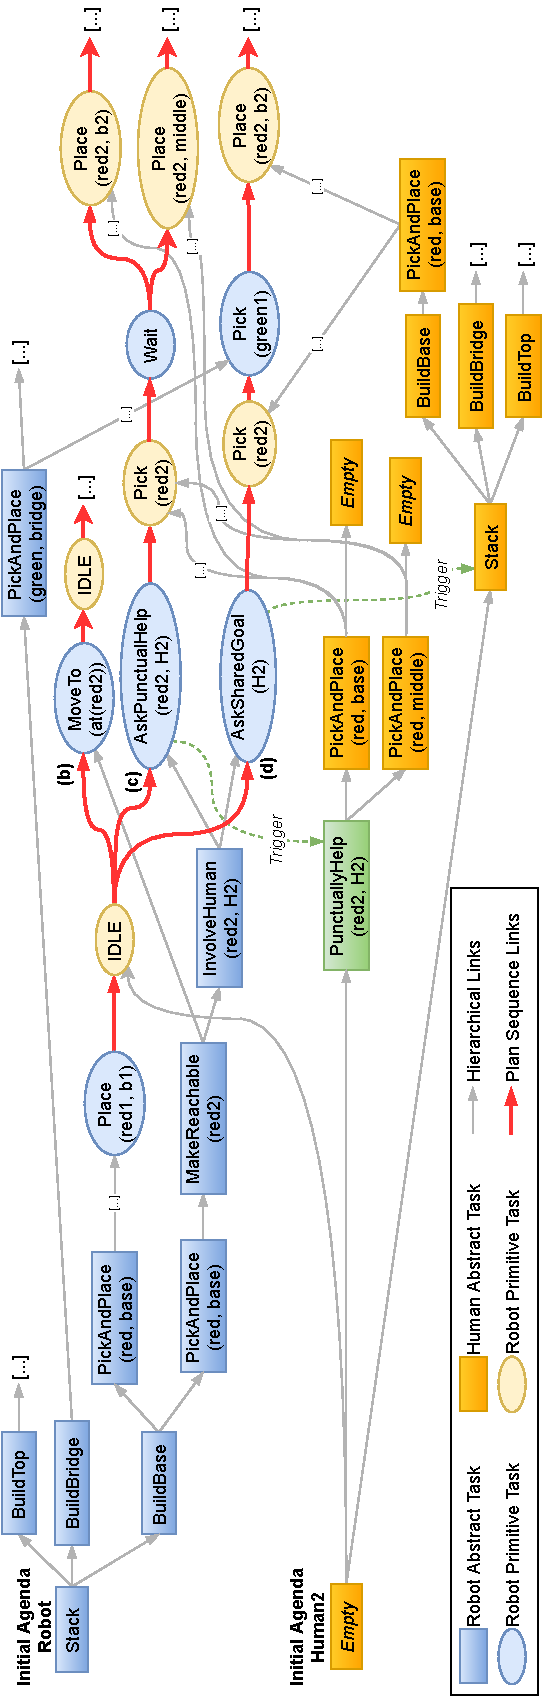
\includegraphics[width=0.45\textwidth]{images/Chapter2/plans_rotated.pdf}
    \caption{Illustration of the incremental exploration of various courses of actions corresponding to scenarios depicted in Fig.~\ref{fig:scenarios}(b), (c) and (d). Since H1 requests the robot to achieve the goal, it is not a shared goal, the robot agenda is filled with the task to achieve and the agenda of H2 starts empty.}
    \label{fig:plans}
\end{figure}

\paragraph{(a) H1 and R act together}
First, the human sets a shared goal by asking the robot to stack cubes with him. Since it is a shared goal, Both human and robot agendas are initialized with the ``Stack" task. Thus, the robot anticipates that the human will pick the unreachable second red cube by querying the human action model. The selected plan to collaboratively stack can be seen in TABLE~\ref{tab:plans}(a). 

\paragraph{(b) Robot acts alone}
This time the human asks the robot to stack the cubes but then leaves the scene, the robot must act alone. Hence, the only applicable method to make the second red cube reachable is to move to the other side even though the movement action is expensive (we can imagine a table way longer than shown on the figure).

\paragraph{(c) Robot asks punctual help}
The first human acts the same way but another one is present, not involved in the task. The robot starts exploring its HTN and, thanks to the presence of the other human, a new method is applicable allowing the robot to ask for help. It can either ask for punctual help or involve completely the other human in the task. Of course, just asking help for one cube is less costly than asking to build the whole stack together. However, asking help to someone not already involved in a common task is still expensive since they have to put themselves in the context of the task. Yet, this punctual help is actually less costly for the robot than moving to the other side so the robot chooses to ask for punctual help. Note that we model the fact that after being asked to punctually help, the human can either stack the cube herself or just make it reachable to the robot by placing it in the middle. Only the first branch is shown in TABLE~\ref{tab:plans}(c) but the selected plan is in fact conditional with two branches as depicted in Fig.~\ref{fig:plans}.

\paragraph{(d) Robot invites Human2 to share a goal}
Same initial setup but now two cubes are out of reach. Asking for punctual help is still less costly than moving around the table. Nevertheless, this disturbs the human so each new punctual request becomes more expensive than before. Thus, this time setting a shared goal becomes less costly for the robot than asking twice for punctual help.

\section{Conclusion}

what is offered by HATP/EHDA is very interesting, we reason on the human model to plan the robot actions while never compelling the human actions. The plan produced assumes Turn-Taking, thus, no parallel execution of the actions. This isn't a strict constraint as a post-analysis can reason on the causal links of the actions in the plan to extract a partially ordered plan to execute, making the execution more flexible. It is however still a limitation that is addressed in Chapter~\ref{chap:4}.